% Drawing 34/09-5 -- folder 34, batch 09, archive page 170 (PDF page 171).
% Transcription: Diagramme de schémas : en haut $X \leftarrow X_K \leftarrow X_{\tilde U}$, en bas $S \hookleftarrow U \leftarrow \bar U$, flèches verticales dans les deux sens (projections et sections) entre $X$ et $S$, $X_K$ et $U$ ; au milieu $X$ (en gras) $\Leftarrow \tilde X$, et $s \leftarrow \bar s$ sous $U$ et $\bar U$ ; à droite, $F_{\bar a}$.
% Kind: diagram of schemes. Method 2 (schematic redraw from the facsimile). Status: partial.
% Notes: Top: X <- X_K <- X_U-tilde; bottom: S <-(hook) U <- U-bar; curved arrows both ways (projections and sections) between X and S and between X_K and U; in the middle a bold X <= X-tilde, with s <- s-bar below; short oblique arrows from X to X_K, from X-tilde to X_U-tilde, from s to U and from s-bar to U-bar; F_a-bar on the right. The B_Gamma ... P square below is typeset in the transcription and is not part of this mark; the long pencil line across the page is left out.
% Coordinates: 1 unit = 1 mm = 1/100 of the crop width (bbox in page fractions: [0.12, 0.47, 0.56, 0.62]).
% Redrawn by Claude (claude-opus-5-5), issue #73, 2026-11-07; not checked by a human; not compiled (no TeX in the session).
% Rights: reproduces part of the work -- behind RENDER_TRANSCRIPTS, never published by itself.
\documentclass[tikz,border=3pt]{standalone}
\usepackage{amsmath,amssymb}
\usetikzlibrary{patterns,arrows.meta}
\tikzset{pencil/.style={black!45}, struck/.style={black!35}, mark/.style={circle,draw,inner sep=1.3pt}, pt/.style={circle,fill,inner sep=0.9pt}, opt/.style={circle,draw,fill=white,inner sep=1.1pt}}
\begin{document}
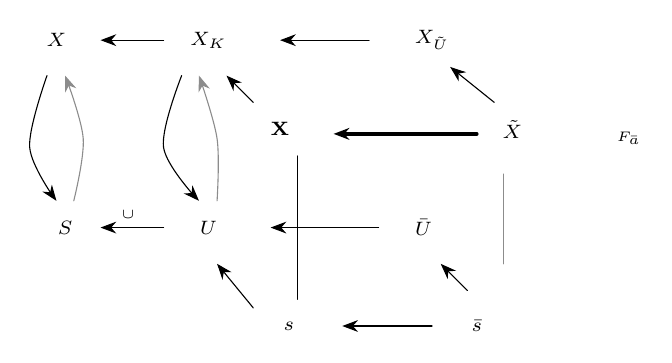
\begin{tikzpicture}[x=1mm,y=1mm,line cap=round,line join=round,font=\scriptsize]
\node[inner sep=1pt] at (23.9,-8.2) {\scriptsize $X$};
\draw[-{Stealth[length=2mm]}] (37.5,-8.2) -- (29.5,-8.2);
\node[inner sep=1pt] at (43.2,-8.2) {\scriptsize $X_K$};
\draw[-{Stealth[length=2mm]}] (63.6,-8.2) -- (52.3,-8.2);
\node[inner sep=1pt] at (71.6,-8.2) {\scriptsize $X_{\tilde U}$};
\node[inner sep=1pt] at (52.3,-19.5) {\scriptsize $\mathbf{X}$};
\draw[-{Stealth[length=2mm]},very thick] (77.3,-20.1) -- (59.1,-20.1);
\node[inner sep=1pt] at (81.8,-19.5) {\scriptsize $\tilde X$};
\node[inner sep=1pt] at (96.6,-20.7) {\tiny $F_{\bar a}$};
\draw[-{Stealth[length=2mm]}] (48.9,-16.1) -- (45.5,-12.7);
\draw[-{Stealth[length=2mm]}] (79.5,-16.1) -- (73.9,-11.6);
\node[inner sep=1pt] at (25,-32) {\scriptsize $S$};
\draw[-{Stealth[length=2mm]}] (37.5,-32) -- (29.5,-32);
\node[inner sep=1pt] at (33,-30.3) {\tiny $\scriptstyle\cup$};
\node[inner sep=1pt] at (43.2,-32) {\scriptsize $U$};
\draw[-{Stealth[length=2mm]}] (64.8,-32) -- (51.1,-32);
\node[inner sep=1pt] at (70.5,-32) {\scriptsize $\bar U$};
\draw[-{Stealth[length=2mm]}] plot[smooth, tension=0.55] coordinates {(22.7,-12.7) (20.5,-21.8) (23.9,-28.6)};
\draw[-{Stealth[length=2mm]},pencil] plot[smooth, tension=0.55] coordinates {(26.1,-28.6) (27.3,-20.7) (25,-12.7)};
\draw[-{Stealth[length=2mm]}] plot[smooth, tension=0.55] coordinates {(39.8,-12.7) (37.5,-21.8) (42,-28.6)};
\draw[-{Stealth[length=2mm]},pencil] plot[smooth, tension=0.55] coordinates {(44.3,-28.6) (44.3,-20.7) (42,-12.7)};
\draw (54.5,-22.9) -- (54.5,-41.1);
\node[inner sep=1pt] at (53.4,-44.5) {\scriptsize $s$};
\draw[-{Stealth[length=2mm]}] (71.6,-44.5) -- (60.2,-44.5);
\node[inner sep=1pt] at (77.3,-44.5) {\scriptsize $\bar s$};
\draw[-{Stealth[length=2mm]}] (48.9,-42.2) -- (44.3,-36.6);
\draw[-{Stealth[length=2mm]}] (76.1,-40) -- (72.7,-36.6);
\draw[pencil] (80.7,-25.2) -- (80.7,-36.6);
\end{tikzpicture}
\end{document}
